\documentclass[twocolumn,11pt]{article}
\setlength{\textheight}{9truein}
\setlength{\topmargin}{-0.9truein}
\setlength{\parindent}{0pt}
\setlength{\parskip}{10pt}
\setlength{\columnsep}{.4in}

\usepackage{amsmath,amsfonts,amssymb,amsthm,bm,caption,calc,ifthen,graphicx,url,hyperref}

\begin{document}
\pagestyle{plain}
\onecolumn
ASTP720 
\newline Homework 5
\newline Will Wainwright
\newline Repository: \href{https://github.com/wjwainwright/ASTP720}{https://github.com/wjwainwright/ASTP720}

\section*{Discussion}
This assignment went a lot faster than most, in part because the tasks we had to do were fewer, but also in part because I had a similar assignment for another class. That being said, I still found enjoyment in applying fitting techniques to data, and I hope to be able to apply these methods to fitting real data in the future.

The assignment said we can justify our fits in whatever way we want, so I looked at the fit in both 2D and 3D, and decided that a 2D fit was representative enough for the purposes of justification. I also compared the parameters that my fit returned to those of the scipy curve fitting method. Both methods returned the same parameters, so that is a signal to me that the method was implemented correctly. When comparing the simple fit and the fit with uncertainty, the only thing that appears to have changed is the estimated uncertainty in the fit parameters. There could have been a change in the returned fit parameters, but they are rounded to two decimal places and no change occurred on those digits. It should be noted that I did all of my fitting in the V band, as it was left up to choice which band we used. 


\begin{figure}[!h]
	\centering
	\noindent
	\makebox[\textwidth]{
      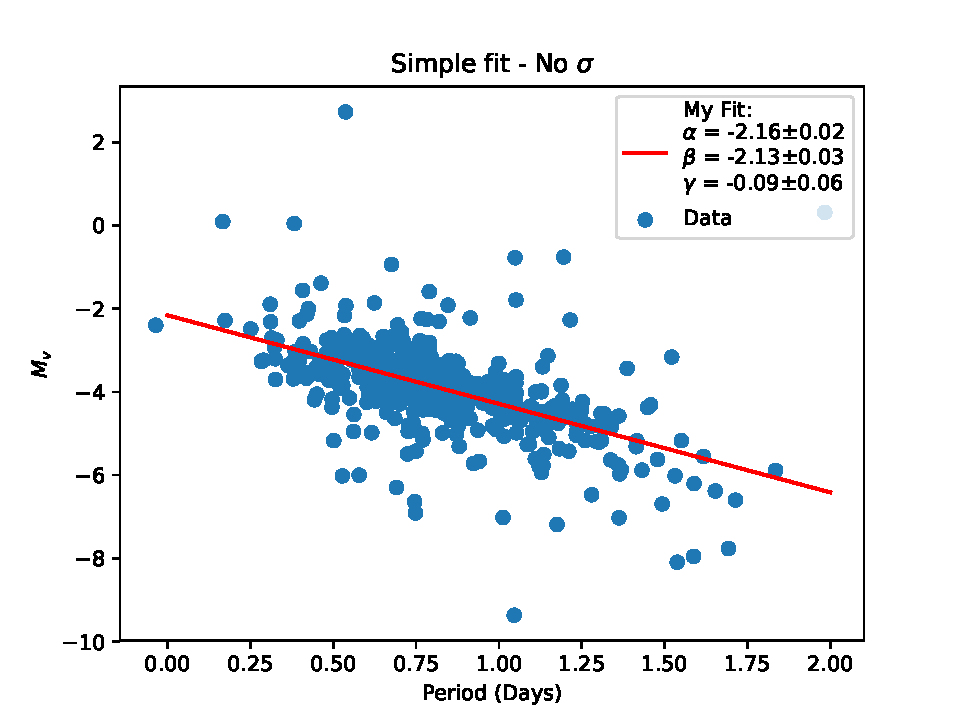
\includegraphics[width=4.5in]{simplefit.pdf}}
      \caption{Fitting the data without any given uncertainty in 2D, ignoring the $\frac{Fe}{H}$ axis that is used to get the fit for $\gamma$.}
\end{figure}

\begin{figure}[!h]
	\centering
	\noindent
	\makebox[\textwidth]{
      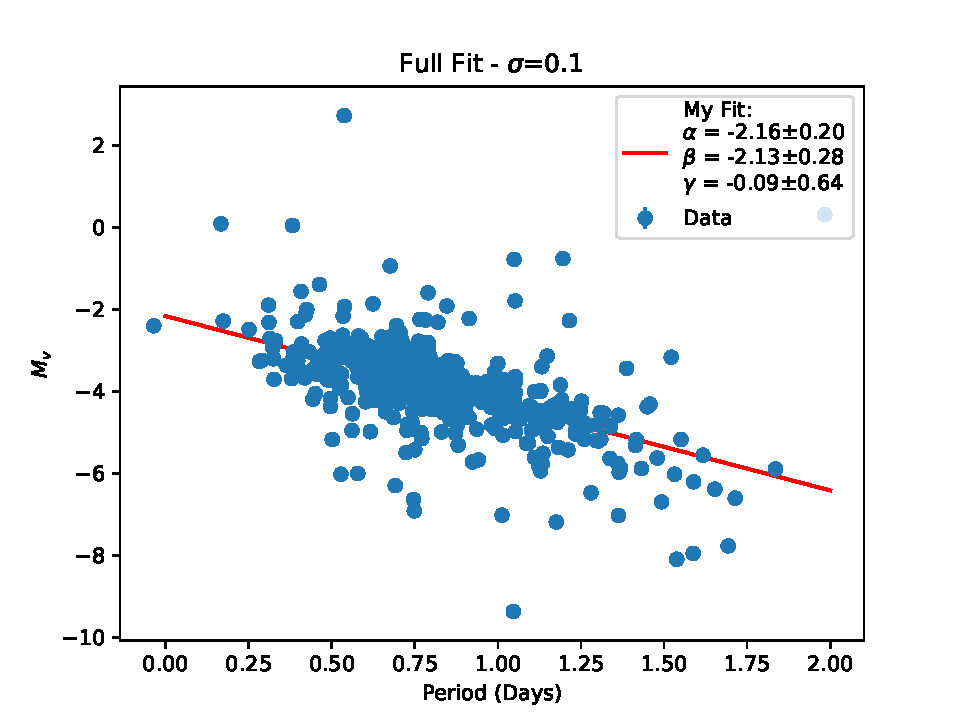
\includegraphics[width=4.5in]{fullfit.pdf}}
      \caption{Fitting the data with an uncertainty of $\sigma=0.1mag$. Notice that the fit parameters do not change but the uncertainty in the fit does change.}
\end{figure}

\begin{figure}[!h]
	\centering
	\noindent
	\makebox[\textwidth]{
      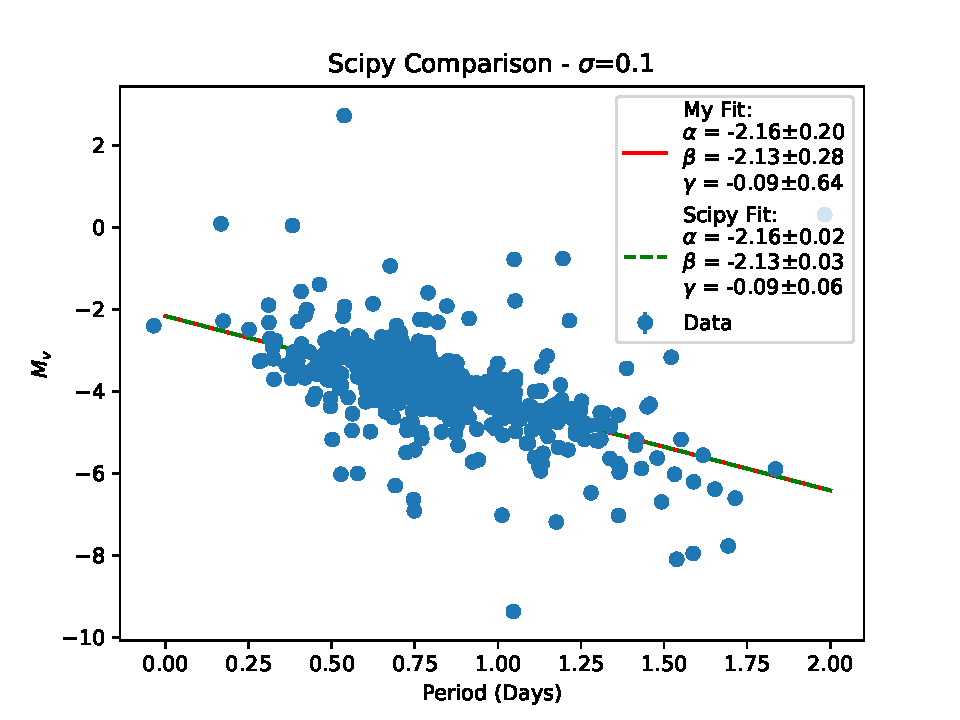
\includegraphics[width=4.5in]{comparison.pdf}}
      \caption{Comparison of my fit to that of scipy's curve fitting method. The fact that both return the same fit parameters gives me confidence in my fit.}
\end{figure}

\begin{figure}[!h]
	\centering
	\noindent
	\makebox[\textwidth]{
      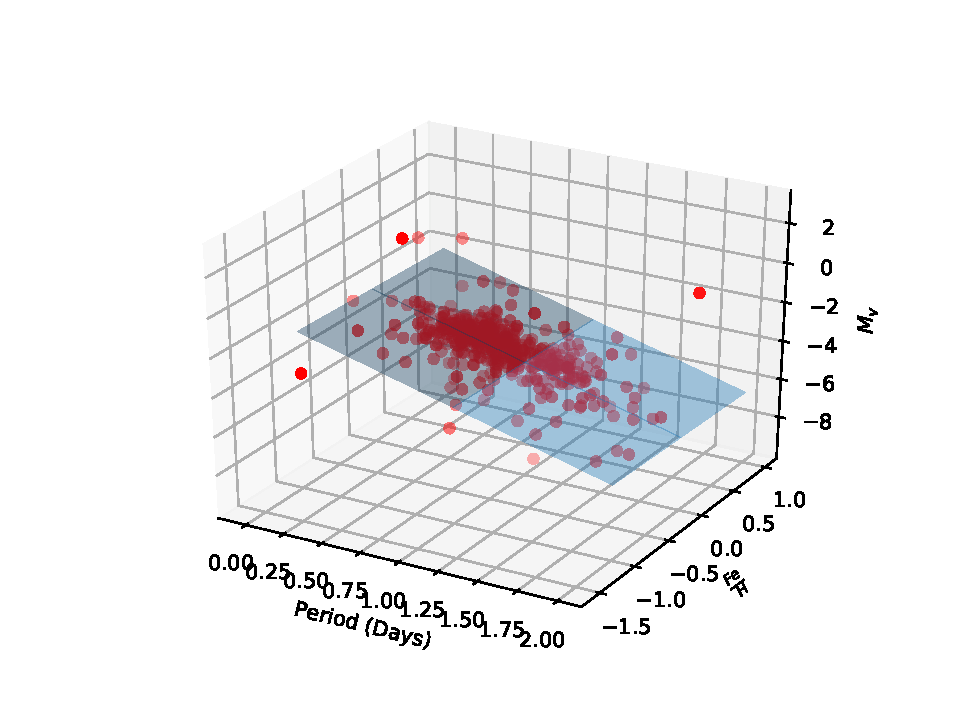
\includegraphics[width=4.5in]{3Dplot.pdf}}
      \caption{3D plot of the parameter space with the best fit represented as a plane. Note that I could only figure out how to fit the plane to one of the three dimensions, so it is not fit to the extra axis compared to the 2D fit, but rather the 2D line fit extended into a third dimension.}
\end{figure}



\end{document}